
\section{Глава 4. Проектирование системы для отправки сообщений на борт дрона с наземной станции}

Отправка видеопотока производится за счет UDP пакетов.  Данный протокол не гарантирует доставку сообщений, но позволяет уменьшить задержку получения потока, что более критично. Проверены кодеки jpeg, h264, omxh264enc, из них самым стабильным по задержке оказался h264. Задержка составила 150 мс.

После включения дрона и загрузки ОС RPi производится удаленное подключение к Raspberry Pi.
Запускается gstreamer для передачи изображения с rpicamsrc на адрес наземной станции UDP пакетами. Команда представлена в листинге \ref{lst:12}:
\begin{Program}[H]
	\caption{Команда запуска gstreamer} \label{lst:12}
\begin{MyCode}
$ gst-launch-1.0 rpicamsrc bitrate=1000000 !\
'video/x-h264,width=640,height=480' ! h264parse !\
queue ! rtph264pay config-interval=1 pt=96 ! gdppay !\
udpsink host=[IP ПК] port=5000
\end{MyCode}
\end{Program}

На наземной станции в первой вкладке консоли запускается окружение mavros (листинг\ref{lst:13} ):
\begin{Program}[H]
\caption{Команда запуска окружения mavros} \label{lst:13}
\begin{MyCode}
$ roslaunch mavros px4.launch
\end{MyCode}
\end{Program}
После того, как произошли подключение и инициализация дрона в окружении, во второй	 вкладке консоли производится сброс координат дрона (листинг \ref{lst:14}):
\begin{Program}[H]
	\caption{Команда сброса координат дрона} \label{lst:14}
\begin{MyCode}
# инициализация параметров SET_GPS_GLOBAL_ORIGIN и SET_HOME_POSITION
$ rosrun aruco_gridboard set_origin.py
\end{MyCode}
\end{Program}
В третьей вкладке консоли запускается aruco\_gridboard, совмещенный с нодой gscam, для получения и обработки изображения (листинг \ref{lst:15}):
\begin{Program}[H]
\caption{Команды запуска aruco\_gridboard с нодой gscam} \label{lst:15}
\begin{MyCode}
$ export GSCAM_CONFIG="udpsrc port=5000 ! gdpdepay !\
rtph264depay ! avdec_h264 ! videoconvert"
$ roslaunch aruco_gridboard detection_rpicam.launch 
\end{MyCode}
\end{Program}

Для проверки корректности работы системы можно запустить программу rviz (листинг \ref{lst:16}):
\begin{Program}[H]
\caption{Команда запуска rviz} \label{lst:16}
\begin{MyCode}
$ rosrun rviz rviz -d catkin_ws/src/aruco_gridboard/data/aruco_grid.rviz
\end{MyCode}
\end{Program}
На рисунке \ref{fig:px4} отображены вывод в консоль координат, полученных aruco\_g\-rid\-board, изображение с камеры дрона с началом координат на карте маркеров и поле rviz с моделью дрона относительно карты.
% ~\ref{fig:px4}
\begin{figure}[H]
	\centering
	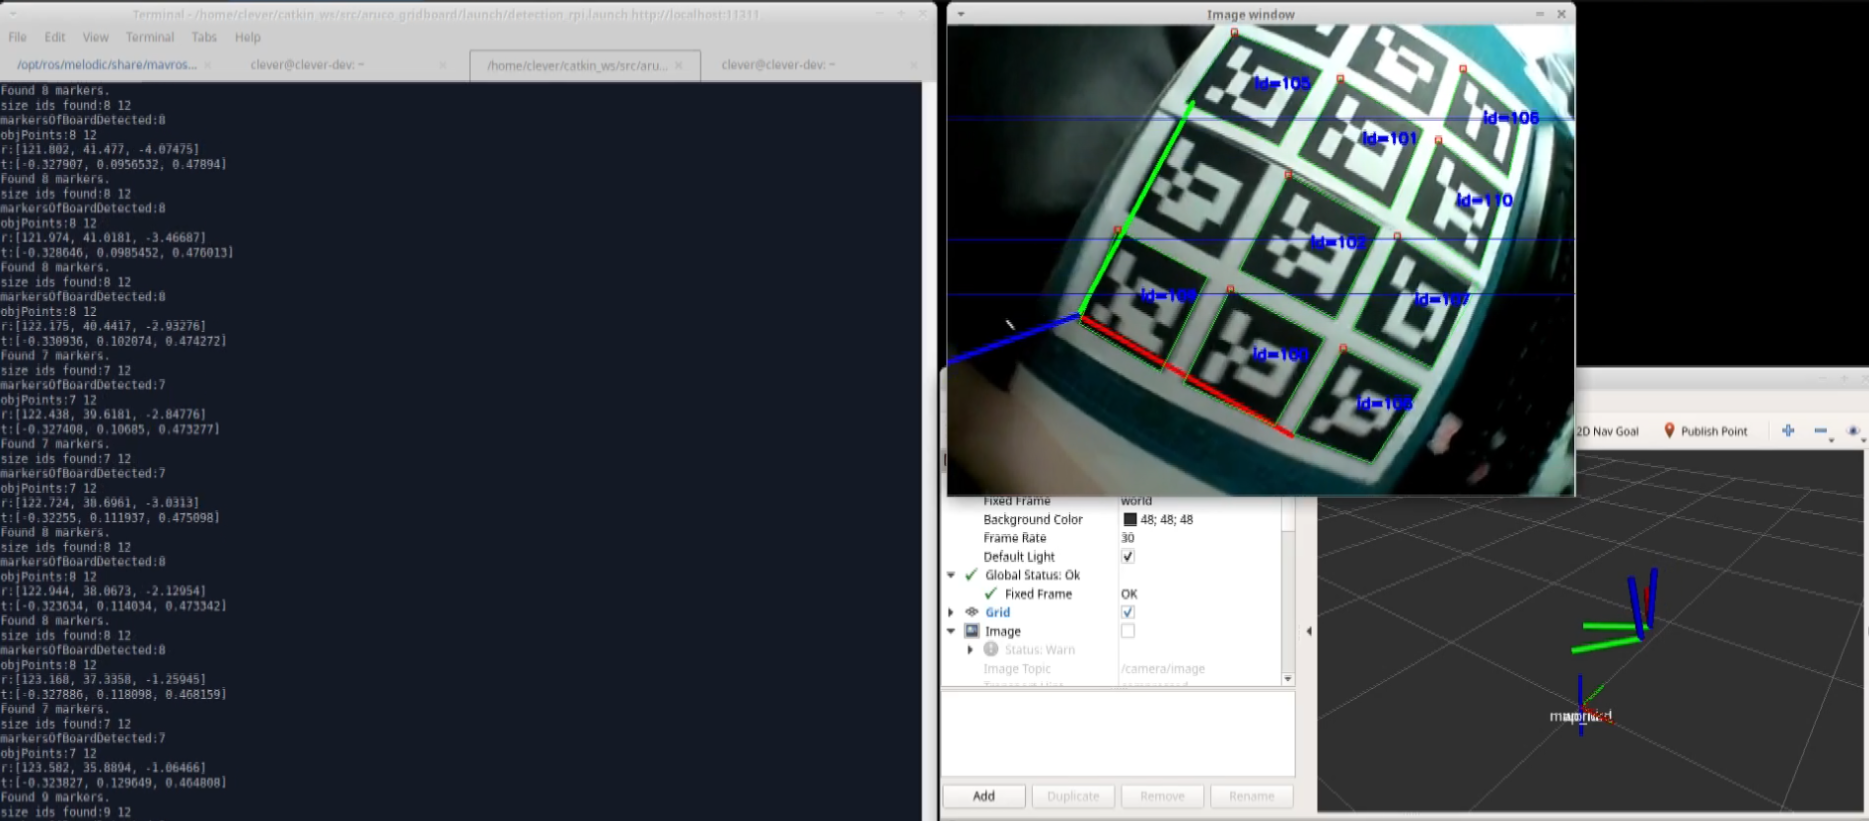
\includegraphics[width=0.9\linewidth]{pics/px4}
	\caption{ Скриншот экрана наземной станции во время определения положения дрона
	}
	\label{fig:px4}
\end{figure}
